\chapter[\paperIItitle]{\texorpdfstring{%
                \paperIItitle}{%
                \paperIItitle}}

\label{ch:ppiot}
\paperRemark{This is the full version of the paper below.
        This version contains an extended background description, and a more detailed motivation behind choices in the implementation as well as evaluation.

        \paperIIref}

{


\section{Introduction}
\label{introduction}
Internet-of-thing (IoT) is a network of physical objects or \emph{things} embedded with electronics, software, and sensors, connected through the Internet to collect and exchange data with manufacturers, operators and other connected devices. IoT includes a variety of connected objects from tiny stuff (e.g. smart dust) to enormous stuff (e.g. an entire city). Most IoT devices are used in factories, businesses and healthcare systems. By 2025, there might be more than 75.4 billion connected devices \footnote{https://www.statista.com/statistics/471264/iot-number-of-connected-devices-worldwide/} 
generating 175 trillion gigabytes of data\footnote{https://www.seagate.com/gb/en/our-story/data-age-2025/}, 
and total global worth of IoT technology would reach to USD 6.2 trillion by 2025\footnote{https://www.intel.com/content/www/us/en/internet-of-things/infographics/guide-to-iot.html}. 
This trend opens up to completely new possibilities with respect to data analysis services utilizing device data from a huge number of distributed devices \cite{Marjani2017}. The applications are very wide-ranging from healthcare and market analytics to industrial systems. In this paper, we consider big data IoT analytics from a privacy perspective. Even if the IoT units producing the data are not necessarily owned by an individual, the data they produce as well as communication patterns can reveal important business and industry secrets which should be avoided whenever possible \cite{Sadeghi2015} \cite{Maple2017}.

Huge scale analytic on powerful, third-party back-end cloud resources raises security and privacy concerns. One problem is that typically the cloud computing resources cannot be fully trusted. Another related problem is that if an adversary is able to observe the analytic operations or data storage read/write requests, sensitive information might be leaked. One way to tackle this problem is to use privacy-preserving cryptographic techniques \cite{Papadimitriou2016} \cite{Popa2011}, \cite{Wang2017}. However, so far these approaches have large overhead and thus severely limits the type of analytic operations that can be supported in the system. Especially the area of fully homomorphic encryption has achieved lots of attentions even if it is not yet fully practical \cite{Acar2018}.  An alternative approach is to operate on original data using analytic engines executed in Trusted Execution Environments (TEEs) such as Intel\textquotesingle s SGX. This line of research has gained quite a lot of attention during the past years \cite{Xu2018}\cite{Zheng2017}\cite{Schuster2015}. In these approaches, it is assumed that the data subject to data analysis is \emph{already} encrypted with a suitable encryption key available to the trusted application running in the TEE. Hence, before these protection techniques can be applied, the database content must be properly encrypted with the expected keys. In a scenario, where a large amount of IoT devices regularly uploads new data items subject to analysis, the data items must also be protected prior to arriving at the cloud storage resources \emph{and} they should be protected \emph{end-to-end}  without leaking any information about the source IoT unit. How to perform such encryption in an identity privacy-preserving and efficient way is the problem tackled in this paper. 

One key difference that needs to be taken into account when designing an IoT system solution is that in many applications, the IoT devices are resource-constrained \cite{Mun2016}.  They can, for instance, be constrained both in terms of computation power, as well as, being energy-constrained since they can be powered by a battery. Besides being more resource-constrained, they are also often deployed in a decentralized manner. These constraints limits, to a varying degree, what kind of security mechanisms that can be put in place, as well as, what kind of algorithms that can be executed on the IoT units \cite{Roman2011}. Hence by efficient, we here mean to avoid the trivial solution using public key encryption, which both is costly on the resource-constrained devices as well as when processing a large number of data items on the cloud resources.

Using a model of the availability of trusted computing engines in the cloud like the solutions in \cite{Zheng2017} and \cite{Schuster2015}, we consider the \textit {additional} and \textit{orthogonal} security problem of privacy preserving data cloud upload of IoT subject to data analysis. Especially, we consider this problem in the context of {\textit not} requiring any public key operation on the data collection, i.e. IoT, side but pure symmetric operations. Furthermore, we require IoT  \textit{individual} symmetric encryption keys as global encryption keys constitute a major security risk (a compromise of a single IoT unit will destroy the security for all or many devices).  In this context, the main challenge is to design a symmetric data encryption scheme allowing fast encryption and decryption while preventing an attacker, observing the data in transfer or at cloud storage, deducing any information bout the data origin like the identity of the IoT unit producing the data. Still, it must be possible for the analytic engines running at the cloud resources to efficiently to decrypt the data. We address this challenge suggesting an data item identity preserving encryption scheme and corresponding key management scheme.

The main contributions of the paper are the following:
\begin{itemize}
    \item We identify main security requirements for large scale, light-weight and identity privacy preserving, individual IoT data encryption and give formal security definitions.
    \item We present a novel encryption and corresponding key management scheme meeting the identified requirements.
    \item We evaluate the security properties of the proposed scheme and prove the security of the scheme for a couple of different attacker scenarios.
    \item We present a proof of concept implementation of the encryption scheme and make a performance evaluation.
\end{itemize}

We proceed as follows: we present the system scenario we are considering (\S \ref{Systemscenario}), we introduce our adversary model and derive security requirements as well as make formal security definitions (\S \ref{requirements}),  we give an overview of our novel IoT data encryption scheme and introduce notations (\S \ref{design}), we describe our proposed key management solution (\S \ref{keymanagement}), we present the detailed data encryption and decryption procedures (\S \ref{dataprotection}),  We make a formal security analysis of the proposed solution (\S \ref{secanalysis}) and present a proof of concept implementation, including performance figures (\S \ref{peranalysis}). Lastly we discuss related work (\S \ref{relatedwork}) and conclude (\S \ref{conclusion}).


\section{System scenario}
\label{Systemscenario}
We consider a system consisting of distributed IoT units, a management domain and a third-party cloud back-end (cloud provider) responsible for IoT data storage as well as data analytic operations.  Figure \ref{fig:systemarchitecture} depicts an overall system scenario which includes the following components: 

\begin{figure*}[th]
    \begin{centering}
    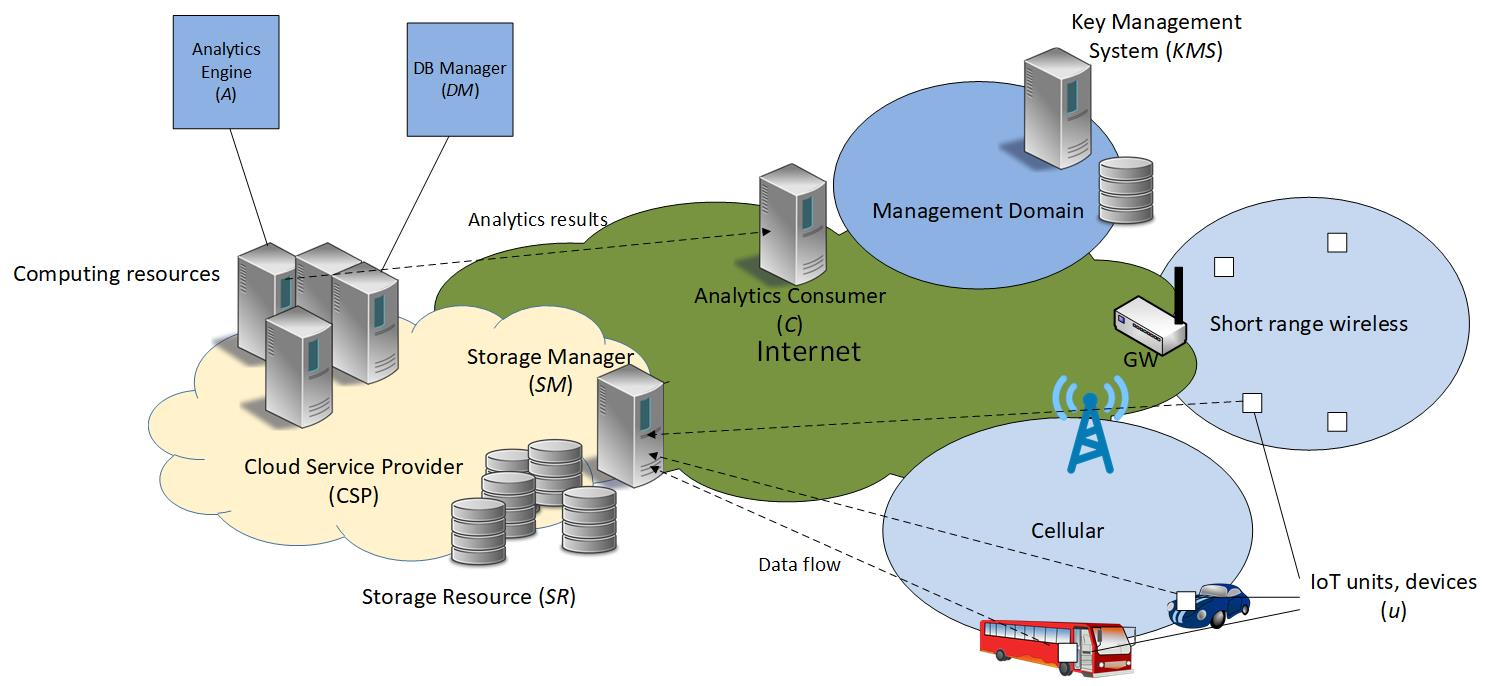
\includegraphics[width=\textwidth]{papers/ppiot/images/SystemArch}
    \caption{System scenario.}
    \label{fig:systemarchitecture}
    \end{centering}
\end{figure*}

%The different introduced components in the scenario and their notations are as follows:
\begin{itemize}
\item The Key Management System ($KMS$) deployed in a management domain is responsible for generating different credentials for IoT units and cloud execution containers, as well as the other entities running at a Cloud Service Provider (CSP) that need key material. The $KMS$ may also collect analytic results. 
\item CSP Storage Resource ($SR$), which is a repository responsible
for storing IoT data. 
\item Storage Manager ($SM$) which is the interface for collecting and accepting IoT data and storing it on the SR.
\item IoT units or what we refer to as devices ($u$) producing data which is sent securely to the SM component. The architecture is agnostic with respect to how the devices are deployed and in what type of network. All devices are assumed to have global network connectivity.
\item Database Manager ($DM$) responsible for sharing IoT data with analytic engines. The DM is deployed in a suitable execution container on the cloud resources in the form of a Virtual Machine (VM) or in a protected execution container like SGX.
\item Analytical engines ($A$) perform data analytics on IoT data through the DM. The analytics engines in the system are deployed on suitable execution containers on the cloud resources in the form of  Virtual Machines (VMs) or in protected execution containers like SGX.
\item Aanalytics consumer ($C$) which is authorized to receive analytics results produced by an A.
\end{itemize}

The boundary of the CSP is the space that contains $SM, SR, DM$ and $A$. The management domain might also be deployed in an cloud environment but must in the model we are considering be fully trusted. We discuss the adversary model and requirements in the next section. 

\section{Problem setting}
\label{requirements}
Next, we discuss the details of the data protection problem we are considering. We start by defining our adversary model and use this model to identify privacy requirements. Although the system scenario and architecture we are considering implies several additional requirements, the focus here are on the privacy/security requirements under the assumption of resource constrained IoT units. Next, we identify security and functional requirements on the system we are considering. Finally, we give formal security definitions. 
\subsection{Adversary model}
\label{requirements:adversary}
We consider a powerful adversary who may control the CSP network domain as well as having access to the $SM$ and $SR$. We do not consider denial-of-service (DoS) types attacks on these nodes though and assume that $SM$ and $SR$ are being able to operate properly. The adversary might also try to get full access to the computing resources but we assume the $A$ and  $DM$ to be deployed in secure containers using secure launch in combination with secure VMs or secure launch of SGX machines. Hence, the adversary has no possibility to directly modify or eavesdrop $A$ or $DM$. This model is motivated, as we stated in the introduction, with reference to trusted computing techniques in combination with secure launch as reported in \cite{Paladi2017} and protected SGX analytics as described in \cite{Schuster2015}. Recent attacks like Metldown \cite{Lipp2018} and Spectre \cite{Kocher2019}  have shown that one cannot even trust the fundamental hardware functions needed for secure isolation currently in use. Despite this fact, the security with respect to secure execution environment for virtualized systems is steadily improving and we will in this paper disregard attacks on the isolation properties of the execution containers. 

In line with many other works on IoT and cloud security, we assume that the adversary is acting according to the Dolev-Yao adversarial model \cite{ Dolev1981}. This implies that an attacker is able to intercept, delete, change order or modify all communication messages sent over the communication links between the IoT units and the CSP domain. The adversary can also destroy messages but is not able to break any cryptographic mechanisms. The devices are assume to be semi-trusted. This means that as long as an external attacker has not compromised a unit, it will be trustworthy. However, we do not exclude the possibility of that a limited set of the IoT units in the system are completely taken over by the adversary. 

The management domain including the $KMS$ is assumed to secure not in the control of the adversary.

\subsection{Requirements}
\label{requirements:requirements}
Starting from the previously presented system architecture and the given adversarial model, we have identified the following security requirements:
\begin{labeling}{R4.}
\item [R1.] \textbf{Data items confidentiality:} All data items sent from a device $u$ needs to be confidentiality protected, all the time, until they are processed by $A$ in a secure execution environment.
\item[R2.] \textbf{Data items integrity:} All data items sent from a device $u$ needs to be integrity protected, all the time, until they are processed by $A$ in a secure execution environment.
\item[R3.] \textbf{Analytics results confidentiality and integrity:} All analytics results must be confidentiality and integrity protected before they are returned to the $C$. 
\item[R4.] \textbf{Data items identity privacy:} It shall not be possible for an external adversary or a compromised IoT unit, $u'$ to determine which data item that is produced by a, non compromised, specific IoT unit, $u$. This implies that it shall not be possible to trace data items from different IoT units through potential identities used in protected data items.
\end{labeling}
Many of the devices might be placed in internal network not accessible from the outside. Furthermore, a particular device, $u$, might for security reasons be restricted not to set up secure sessions with external entities. It might also be an advantage if several data items can be buffered at an intermediate node, before they are transferred to the $SM$ for storage. Altogether, this gives us the following additional design requirement on the wanted solution:

\begin{labeling}{R5.}
\item [R5.] \textbf{IoT unit isolation:} A data transfer from $u$ shall not require any direct interactions (session) between the IoT unit and the $SM$.
\end{labeling}
Among these, requirements, it is particular challenging to fulfill requirement R4 in combination with R1 and R2 for the scenario we are considering. This is due to the fact, that it shall be possible for analytic engines deployed in the cloud, to quickly decrypt data items uploaded to the cloud using symmetric encryption only. This on the other hand, requires that the symmetric key for the data items must be available which in turn typically means that the data item must be ''marked'' with a key identity to allow symmetric key lookup. If a fixed identity is used, we do not fulfil R4 and this is the main security design challenge we address in this paper.

\subsection{Formal security definitions}
\label{requirements:secdefinitions}
Next, we give formal security definitions. We here focus on formally defining R1, R2 and R4. The reason for this choice  is that R3 can be fulfilled with standard secure channel and security association techniques and it is not the main problem we address here even this is a requirement for  a complete system solution. Furthermore, R5 is not a security requirement as such, but a property on the solution we want to have in order to offer practical and broadly applicable solution. Hence, we here do not either give a formal definition for R5.

Denote by $u\in U$ an arbitrary IoT unit and by $m \in M_n$, where $M_n$ is a plain text space index by $n$ (message of length $n$ bits), a data item produced by such unit. Furthermore, let $K_e \in {\cal{K}}_e$  and $K_{mac} \in {\cal{K}}_{mac}$, be a symmetric encryption and integrity keys respectively, known to the $u$ and the $DM$. We then denote by $c = E_{K_e}(r,m)$ the encryption of $m$ with Initialization Vector (IV) $= r \in R$ and using a suitable symmetric encryption algorithm, $E$. Similar, we denote by $x = \text{MAC}_{K_{mac}}(m)$, the message tag calculation for a message, $m$, using a suitable MAC function , MAC\footnote{In the scheme we consider the encryption and message authentication message scopes are not always the same. However, for simplicity, we here just use the notion of $m$ for the message input both to a encryption function and a MAC function}.

Let $K$ be an arbitrary key space and $v = f_K(u,m), K\in \cal{K}$ be the random packaging of message $m$ for unit $u$. Here the function $f_K$ denotes the combination of one or several encryption and/or MAC functions for a particular unit. $v$ is then the actual message ''observed'' by an external entity when the message is transferred to SM.

We use the classical security by indistinguishability definition to define the expected confidentiality property of the scheme \cite{Golrdreich97}.
\begin{definition}
\label{confidentiality}
An IoT protection schemes provides \emph{confidentiality protection} if for all (non-uniform) polynomial time limited  adversaries, $AT$, there exist a negligible function $\epsilon(n)$, such for all $\forall m_0,m_1 \in M_n, \forall r \in R$: 
\begin{eqnarray}
     &&|Pr[AT(E_{K_e}(r,m_0)) = 1] - Pr[AT(E_{K_e}(r,m_1)) = 1]| \nonumber \\ 
     &&< \epsilon(n), \label{req:eqconfidentiality}
     \label{eq:confidentiality}
\end{eqnarray}
where the probability is taken over all choices of $K_e$ and coin tosses by $AT$.
\end{definition}
Let the adversary, $AT$ having access to $\text{MAC}_{K_{mac}}$. We then consider the following security game (unforgeability under chosen message attack):
\begin{itemize}
    \item[] Game UF-CMA \\
    \item Setup: $K_{mac} \leftarrow_R {\cal{K}}_{mac}$
    \item Query phase: $AT$ makes a set of quires, by selection of message $m \in M$ to get $x = \text{MAC}_{k_{mac}}$
    \item Guess phase: $AT \rightarrow (m',x')$
    \item Verify: If $m' \notin M$ and $x' = \text{MAC}_{K_{mac}}(m')$, $AT$ wins, else $AT$ loose.
\end{itemize}
We then use the classical unforgeability MAC security definition for message integrity security.
\begin{definition}
\label{Macunforgeable}
A family of functions, $MAC$, is said to be $(q,l,\epsilon)$ unforgeable  under  chosen  message attack if for all adversaries, $AT$ who makes $q$ queries with total size of the queries bits maximum equal $l$: 
\begin{eqnarray}
     Pr[AT\: \text{win  game UF-CMA}] \leq \epsilon \label{req:integrity}
\end{eqnarray}
\end{definition}
\begin{definition}
\label{integrity}
An IoT data protection scheme which protects messages by a $(q,l,\epsilon)$ unforgeable MAC is said to provide \textit{integrity protection} if $q$ is greater than the maximum number of MAC values that the attacker can observe from a single IoT unit, $\epsilon$ i negligible and $l$ is greater than the maximum number of bits in $d$, i.e, the maximum number of bits produced by any IoT unit for a single message.
\end{definition}
Next, we give our identity privacy definitions. Now, let the adversary, $AT$ having access to the output of $f_{k}$. We consider the following security game (Identity attack):
\begin{itemize}
    \item[] Game IDA \\
    \item Setup: $K \leftarrow_R \cal{K}$
    \item Query phase: $AT$ makes a set of queries to get $v = f_K(u,m)$ together with $u$ for random $u \in U$ and chosen message $m \in M$.
    \item Observe phase: For random $\hat{u}$ and chosen $m \in M$, $AT$ observes  $v' = f_K(\hat{u},m)$
    \item Guess: $AT \rightarrow u'$
    \item Verify: If $u' =  \hat{u}$, $AT$ wins, else $AT$ loose.
\end{itemize}
\begin{definition}
\label{idprivacy}
A data and identity protection scheme, $f$, is said to be $(q,p)$ unforgeable if for all adversaries, $AT$ who makes $q$ queries: 
\begin{eqnarray}
     Pr[AT\: \text{win  game IDA}] \leq p \label{req:privacy}
\end{eqnarray}
\end{definition}
Furthermore, we say that a $(q,p)$ unforgeable protection scheme with $p \leq 1/k$, for an integer $k$, provides \textit{k-anonymity}. 
%Privacy-preserving distributed k-anonymity \cite{JiangC05}

\graphicspath{{DesignOverview/images/}}
\section{Design overview and notations}
\label{design}
Our goal is to provide confidentiality, integrity and identity privacy of cloud uploaded data items. The goal with the design has been to use, due to resource consumption reasons, pure symmetric key algorithms and without any requirement on session handling at the IoT side and with individual encryption keys on the IoT side avoiding that a single or few compromised IoT units will destroy the security of the complete system.

Our solution is based on the following assumption:
\begin{itemize}
\item Referring to solutions like the one presented in \cite{Schuster2015} \cite{Paladi2017}, a trusted analytics provider is able to securely launch analytics applications ($A$) as well as a database manager ($DM$) on secure/isolated VM/containers on the CSP computing resources. The DB server is working on encrypted data stored at general available storage resources ($SR$) in the provider cloud. 
\end {itemize}
We suggest a solution where the $DB$ server is pre-configured (prior to secure launch) with IoT data item symmetric key material that will allow it to read encrypted data items stored on the provider storage resources. Similarly, all IoT units are pre-configured with matching (but not the same) symmetric key material allowing them to upload or release (for instance through a third entity in the local network) encrypted data items to the provider storage resources.

Data items are directly or indirectly uploaded to the storage resources ($SR$) through the $SM$ in the provider network. The solution is agnostic with respect to how the data items are uploaded to the $SM$. The encryption of the data items are done so that an attacker who only observes stored or sent data items neither can obtain the clear text of the individual data items nor being able to know which particular IoT node that uploaded the protected data item. 
 
Once a set of new data items are uploaded to the provider storage resource, the $DM$ is able to immediately fetch any new items, and with low computational overhead (only symmetric encryption), decrypting these items. When the items have been decrypted, the $DM$ updates the internal database index such that efficient search of the data items are possible. The $DM$ server keeps the index in internal protected memory and/or in protected external non-volatile memory.

The data analytic application, or applications, can contact the $DM$ through a protected channel to issue database quires on the encrypted data items. The $DM$ server then efficiently fetches encrypted data items using the internal index and the clear text of the data items are obtained using the symmetric encryption scheme together with the shared (with the IoT units) key management scheme.

Table \ref{tab:notations} summarizes the notations we use throughout the rest of the paper.

\begin{table}[th]
\caption{Notations.}
\label{tab:notations}
\begin{tabular}{||l|l||} \hline
$U$ & Set of devices in the system \\ \hline
$|U|$ & Cardinality of set $U$ \\ \hline
$\{U_0, U_1,\cdots, U_{q-1}\} = U$ & Set of $q$ distinct subsets of $U$ \\ \hline
$u \in U$ & A device in the system \\ \hline
$i$ & Device index \\ \hline
$t$ & Group index \\ \hline
$u_i$ & Device with index $i$ \\ \hline
$d$ & Data item produced by a device \\ \hline
%$(Pr_{PMS},Pu_{PMS})$ &  Private, public key pair of the $kMS$ \\ \hline
%$Cert_{PMS}$ & Certificate certifying $Pu_{kMS}$ \\ \hline
%$(Pr_{DM},Pu_{DM})$ &  Private, public key pair of the $DM$ \\ \hline
%$Cert_{DM}$ & Certificate certifying $Pu_{DM}$ \\ \hline
%$(Pr_{A},Pu_{A})$ &  Private, public key pair of the $A$ \\ \hline
%$Cert_{A}$ & Certificate certifying $Pu_{A}$ \\ \hline
$IK$ &  System wide integrity protection key \\ \hline
$KM1$ & First symmetric master key \\ \hline
$KM2$ & Second symmetric master key \\ \hline
$KM3$ & Third symmetric master key \\ \hline
$IK_i$ & Device unique integrity protection key \\ \hline
$K1_i$ & First device unique encryption key \\ \hline
$K2_i = K2_t$ & Group unique, \\
& second device encryption key \\ \hline
$IV1$  & First Initialization Vector (IV) \\ \hline
$IV2$ & Second IV \\ \hline
$c1$ & First ciphertext \\  \hline
$c2$ & Second ciphertext \\ \hline
$h_o$ & Outer message authentication tag \\ \hline
$h_{in}$ & Inner message authentication tag \\ \hline
$r,n1,n2$ & Random numbers \\ \hline
$||a|| $ & Size of parameter $a$\\ \hline
$a||b$ & Concatenation of value $a$ and $b$ \\ \hline
$L_i = \{{l_i}_0, {l_i}_1,\cdots, {l_i}_{w-1}\}$ & Set of indices given to unit $u_i$ \\ \hline
$\text{E}_K(a,m)$ & Symmetric encryption of message $m$ \\
& with key $K$ and IV = $a$. \\ \hline
$\text{D}_{K}(a,c)$ & Decryption of ciphertext $c$ \\
& using key $K$ and IV = $a$\\ \hline
$\text{MAC}_K(m)$ & Message authentication code for \\
& key $K$ and message $m$ \\ \hline
PRF(K,a) & A Pseudo Random Function taking a \\ 
& key $K$ and additional data, $a$, as input \\ \hline
\end{tabular}
\end{table}

\graphicspath{{KeyManagement/images/}}
\section{Key generation and distribution}
\label{keymanagement}
Next, we describe the principles for key generation and distribution in the system. According to our design, the $KMS$ is responsible for generating keys and to distribute them to the IoT units as well as the DB manager ($DM$), analytic engine ($A$) and storage manager ($SM$) in the system. 

The design is based on the usage of four different master keys: $IK, KM1, KM2$ and $KM 3$. The $IK$ is a system global integrity protection key and the other keys different encryption master keys. Before system deployment, the $KMS$ uses a good random source to generate these four different keys. The key $IK$ is securely transferred and stored at $SM$ while $KM1, KM2$ and $KM3$ are all securely transferred to the $DB$.

To give a k-anonymity on visible device index, the set of IoT units, $U$, is divided IoT subsets of at least size $k$:
\begin{eqnarray}
\label{keygen:deviceset}
U = \{U_0,U_1,\ldots, U_{s-1}\}, \forall t, 0 \leq t \leq s-1, |U_t| \geq k.
\end{eqnarray}
Each IoT unit is associated with a random index, $i$ selected by the $KMS$. $i$ is configured into the $DB$ together with the rest of the key material but is \emph{not} given to the device ($u$) itself. Instead, each device $u_i \in U$ is given a device unique index set:
\begin{eqnarray}
\label{keygen:devindex}
L_i = \{{l_i}_0, {l_i}_1,\ldots, {l_i}_{w-1}\}, l_{ip} = r||\text{E}_{KM3}(r,i),
\end{eqnarray}
where $r$ is chosen uniformly and at random by the $KMS$ and $\text{E}_{KM3}$ is suitable symmetric encryption function. The device uses the index to "mark" data items produced by the item (see Section \ref{dataprotection} for the detailed data protection procedure). In addition, $u_i$ is  configured with \emph{three} different symmetric keys:
\begin{itemize}
    \item $IK$: the global integrity protection key.
    \item $IK_i = \text{PRF}(KM1, "MAC"||i)$: an individual integrity protection key.
    \item $K1_i = \text{PRF}(KM1,"Enc"||i)$: a symmetric \emph{inner} encryption key
    \item $K2_i = K2_t = \text{PRF}(KM2,t)$: a symmetric \emph{outer} encryption key
\end{itemize}
Figure \ref{fig:keydist} gives an overview of the different key configurations done during system deployment. 
\begin{figure}[ht]
    \centering
    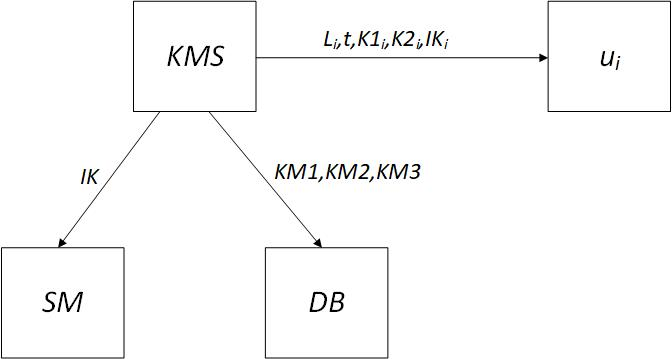
\includegraphics[width=200pt]{papers/ppiot/images/KeyDist}
    \caption{Deployment key configurations.}
    \label{fig:keydist}
\end{figure}

\section{Data protection}
\label{dataprotection}
We are considering a model where a huge number of IoT devices regularly uploads new data items to the storage server $SM$. According requirement R5, this shall be possible to do without the need for any security sessions. A straight forward way to handle this is to use an object security model. Object security for the IETF session protocol for constraint devices, CoAP \cite{rfc7252} is standardized in the Object Security for Constrained RESTful Environment (OSCORE) standard \cite{RFC8613}. While this is a very resource efficient protocol, it gives not identity anonymity of the sending party. Furthermore, it is closely aligned to the CoAP protocol. In our scenario, we do \emph{not} want to just protect the data from the sending device to the storage manager end-to-end as offered by OSCORE, but actually \emph{also} data storage at the $SR$ as we considering a model where the attacker might have access to both the $SM$ and $SR$. Hence, we have defined a new privacy preserving object security format. The format is completely independent of the actual bearer protocol but can for instance be transferred over CoAP as standard non-protected payload. Below, we describe the encryption procedure (at the device side) and format as well as decryption procedures (database side of the system).

\subsection{Data encryption procedure}
\label{dataprotection:encryption}
Each devices regularly uploads data to the $SM$ in protected format. We suggest the following encryption procedure:
\begin{enumerate}
    \item $u_i$ uses a good random source to generate two random values: $n_1,n_2$.
    \item $u_i$ selects uniformly and at random an index, $l_{ip}$, from the set $L_i$.
    \item $u_i$ selects a first encryption IV, $IV1 = l_{ip}||n_1$.
    \item $u_i$ selects a second encryption IV, $IV2 = t||n_2$.
    \item $u_i$ encrypt the data item, $d$ to obtain a first ciphertext: $c1 = \text{E}_{K1_i}(IV1,d)$.
    \item $u_i$ encrypt $IV1$ to obtain a second ciphertext: $c2= \text{E}_{K2_i}(IV2,IV1)$.
    \item $u_i$ compute inner message authentication code: $h_{in} = \text{MAC}_{IK_i}(IV2||c2||c1)$           
    \item $u_i$ calculates a message authentication code over $IV2||c2||c1||h_{in}$: $h_o = \text{MAC}_{IK}(IV2||c2||c1||h_{in})$.
\end{enumerate}
Finally, $u_i$ sends the protected message, $IV2||c2||c1||h_{in}||h_o$, using an arbitrary communication channel to $SM$, which verifies the message authentication tag, $h_o$, and if the verification is successful, stores $IV2||c2||c1||h_{in}$ for future processing at $SR$. The protected message format is illustrated in Figure \ref{fig:protection}.
\begin{figure}[ht]
    \centering
    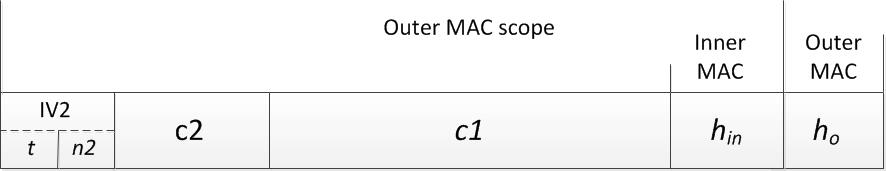
\includegraphics[width=200pt]{papers/ppiot/images/ProtectionFormat}
    \caption{Protection format.}
    \label{fig:protection}
\end{figure}
\subsection{Data decryption procedure}
\label{dataprotection:decryption}
According to the system scenario we are considering, the $DB$ is responsible for decryption protected IoT data items on $SR$ and to index them for future processing. However, there is no need for the $DB$ to re-encrypt the data items but they can be kept in protected form on the $SR$ as the decryption process is quick as we show below.
The decryption procedure is as follows:
\begin{enumerate}
    \item $DB$ fetches a protected data item from the $SR$:  $IV2||c2||c1|h_{in}$
    \item $DB$ extracts $t$ from $IV2$.
    \item $DB$ calculates: $K2_t = \text{PRF}(KM2,t)$.
    \item $DB$ decrypts $c2$ to obtain: $IV1 = D_{KM2}(IV2,c2)$.
    \item $DB$ extracts $l = r||c$ from $IV1$.
    \item $DB$ obtains the true device index $i$ through decryption: $i = \text{D}_{KM3}(r,c)$ (corresponding to the index encryption in (\ref{keygen:devindex})).
    \item $DB$ calculates $KI_i = \text{PRF}(KM1,"MAC"||i)$.
     \item $DB$ calculates $h'_{in} = \text{MAC}_{IK_i}(IV2||c2||c1)$. If $h'_{in}$ equals $h_{in}$, the data, the item is accepted, otherwise it is rejected.
    \item $DB$ calculates $K1_i = \text{PRF}(KM1,"Enc"||i)$.
    \item $DB$ uses $K1_i$ and $IV1$ to obtain the clear text data item $d' = \text{D}_{K1_i}(IV1,c1)$ .
    
    
\end{enumerate}

\graphicspath{{analysis/images/}}
\section{Security analysis}
\label{secanalysis}
Next, we analysis the security properties of the proposed protection scheme. The focus of the analysis is the security requirements R1, R2 and R4 (see Section \ref{requirements:requirements}). R3 is here omitted as this is a pure back-end system property that can be achieved by state-of-the-art protection mechanisms.
\newtheorem{prop}{Proposition}
\begin{prop}
\label{analysis:confidentiality}
 Given that the symmetric encryption algorithm, E, provides confidentiality protection and for a non-compromised IoT unit encryption key, $K1_i$, the proposed scheme provides confidentiality protection.
\end{prop}
\begin{proof}
The worst case attack scenario given the prerequisites in the proposition, is when the attacker has full knowledge of $IV1$ but no knowledge of the key $K1_i$. In this case, for all different data items, $d_0$, $d_1$ and corresponding encrypted cipher texts, $c_0=E_{K1_i}(IV1,d_0), c_1=E_{K1_i}(IV1,d_1)$, the distinguish probability (\ref{eq:confidentiality}) equals the very same probability for the used symmetric encryption algorithm. This proofs the Proposition.
\end{proof}
According to our attacker model, adversary knowledge of $K1_i$ only happens when the IoT unit $u_i$ is compromised. However, if this IoT input is compromised, the attacker will have access to all data protected by this particular unit anyway, and our any protection scheme is not useful. Hence, we conclude that the proposed scheme give good protection for the data for the \textit{majority} of the IoT units. This is true as we assume it will only be feasible for an attacker to compromise a limited number of the IoT units in the system.
\begin{prop}
\label{analysis:integrity}
For a non-compromised IoT unit $u_i$, given that the chosen function $MAC$ is $(q,l,\epsilon)$ unforgeable, the proposed scheme provides data item integrity if: $l $ is greater than the maximum number of bits in $d$, $q$ is larger than the maximum number of messages produced by $u_i$ and $\epsilon$ is negligible.
\end{prop}
\begin{proof}
A data item produced by $u_i$ is first encrypted into $c_1$, which in turn is protected by $(q,l,\epsilon)$ unforgeable $MAC$ using key $IK_i$. Hence, if $IK_i$ is not compromised. $d$ is (indirectly) protected by a $(q,l,\epsilon)$ unforgeable $MAC$. Furthermore, it follows from the assumptions in the Proposition that $l$ is greater than the maximum number of bits in $d$, that $\epsilon $ is negligible and that $q >$ maximum number of messages produced by $u_i$. Hence, the Proposition follows directly from Definition \ref{integrity}
\end{proof}
The same reasoning around IoT encryption key compromise, $K1_i$ for unit $u_i$ applies also to integrity key compromise, $IK_i$ of the unit. Hence the scheme also give good integrity data protection for the \textit{majority} of the IoT units. 
\begin{prop}
\label{analysis:kanonymity}
 Given that the symmetric encryption algorithm, E, provides confidentiality protection and for a non-compromised group encryption key, $K2_t$, the proposed protection scheme provides k-anonymity.
\end{prop}
\begin{proof}
 In the IDA game, the attacker, for chosen messages $m \in M$ observes $q$ different evaluations of  $f_{K2_i}(u_i,m) = c1,c2,h_{in}$ together with $u_i$. Here we have, $c2 = \text{E}_{K2_t}(IV2,IV1)$, where $IV1$ is an encrypted index, $l_{ip}$ randomly mapped from random selections of $u_i$. As the input to the calculation of $c1,c2$, and consequently, also the input to the calculation of $h_{in}$ are depending on random numbers $n1,n2$, these values are randomly distributed on the encryption and MAC spaces independently of the chosen message, $m$. Next, the attacker can choose any previously observed value $t$ (part if $IV1$) and corresponding previously observed message $m$ and get the corresponding, $v' = c1',c2',h'_{in}$. If $c1',c2'$ equals a previous observed $c1,c2$, the attacker wins with probability one as he/she can choose, in this case, a previously observed, $h_{in}$. This probability is less than  the probability that just $c2'$ equals a previously observed crypto text $c2$.  Due to the random selections of $n1$, $n2$, $l_{ip}$ by the IoT unis, observation of a previously observed $c2$ happens with probability less than $2^{\text{log}_2(q) - \text{log}_2(w) - \text{log}_2(||n1||) -\text{log}_2(||n2||)} = \epsilon$. If, $c2'$ does \textit{not} equal a previously observed crypto text, an attacker that tries to decrypt $c2'$ to obtain $l'$, can in the worst case map $l'$ to a particular user $u'$. However, since, the group key, $K2_2$, not is known to the attacker, and the encryption algorithm gives confidentiality protection, it follows from (\ref{eq:confidentiality}) that this attack game succeeds with a probability of at most $\epsilon(n)$. Hence, in case of that $c2'$ does not equal a previous observed crypto text, a random selection of $u' \in U_t$ (as $t$ is known to the attacker) gives the best chance of success. As $|U_t| \leq k, Pr(u'= \hat{u}) \leq 1/k $, this gives an overall probability of success $\epsilon +(1-\epsilon)\cdot(1/k) \approx 1/k$.
\end{proof}
This proposition shows that as long as the group unique key not is leaked, the scheme provided k-anonymity. However, as the size of a group can be rather large  (equal to $t$), compromise of this key cannot be excluded in same cases. However, even in this situation, the proposed scheme gives some anonymity guarantees as showed by the following proposition.

Now, denote by $\text{Bin}(q; k/|U|)$ the binomial distribution, i.e. with the density function:
\begin{eqnarray*}
P(X=j) = 
\begin{pmatrix}
q \\
j
\end{pmatrix}
(k/|U|)^j(1-(k/|U)^{q-j}.
\end{eqnarray*}
Then let: 
\[
 \text{BSum}[(k,w),\text{Bin}(q;k/|U|)] =
 \]
 \[
\begin{cases}
\sum\limits_{j=0}^{q} \frac{1}{k-\frac{j}{w}} P(X=j), & \text{if} \ q \leq w(k-1) \\
\sum\limits_{j=0}^{w(k-1)}\!\frac{1}{k-\frac{j}{w}} P(X=j) + \!\!\!\!\!\! \sum\limits_{w(k-1)+1}^q \!\!\!\!\!P(X=j) & \!\text{otherwise}
\end{cases}
\]
\begin{prop}
\label{analysis:idunforgeable}
Assume, $q < w|U|$, then the proposed protection scheme is \\  $(q,q/(w|U|+(1-q/w|U|)\text{BSum}[(k,w),\text{Bin}(q;k/|U|)])$ unforgeable. 
\end{prop}
\begin{proof}
A worst case scenario is an attacker with full knowledge of $K2_t$ for all possible choices of $t$. Under these circumstance, the attacker can ask for $q$ number of different values $f_{L_i}(u_i) = IV1 = (l_{ip},n_1)$  together with $u_i$ (outer encryption and message selection can be disregarded in this case). Next, in the game, the attacker observes $v' = f_{L_i}(\hat{u})$. If $v'$ has been previously observed, the attacker wins the game with probability one. For each data protection occasion at most $q$ different $(l_{i}, u_i)$ pairs have been recorded by the attacker. Furthermore, as $\hat{u}$ is selected at random \textit{and} the index $l_{i}$ is chosen at random among the $w$ different available indices, the probability that $v'$ has previously been observed is then less than $q/(w|U|)$. This follows from the fact that the total number of $(l_{i}, u_i)$ pairs equals $w|U|$ and that maximum $q$ unique different pairs have been observed by the attacker. If $v$ has not previously been observed, an optimal game strategy for the attacker is to choose $u'$ as the identity of the least number of previously observed identities in $\{v'\}$ belonging to set $U_t$. Denote this number by $z$.  Furthermore, assume, the number of observed elements $U_t$ equals $j$. Then the probability of successful attack for this strategy is less than $(w-z)/(wk-j) \leq w/(wk-j) = 1/(k-(j/w))$, if $j\leq w(k-1)$. While if $j>w(k-1)$, the probability is less than 1. The probability of having $j$ elements in the previous observation belong to set $U_t$ is due to the random selections, equal to the binomial density function. Hence, by taking the expected value of $1/(k-(j/w))$ for the binomial distribution and summing up to the number of observations, $q$, we end up with the an expected probability which is less than $\text{BSum}[(k,w),\text{Bin}(q;k/|U|)]$.
\end{proof}
This proposition is proved under the scenario that all keys $K2_t$ are leaked which is typically not possible to achieve for a limited attacker. Even under this circumstance, as the proposition shows, the scheme still provides a level of anonymity. The strength of the anonymity can be tuned using the size of the parameter $w$. However, a larger $w$ comes with higher IoT non-volatile memory cost. It is important to also notice though, that unforgeability is made under the worst chosen message attack scenario and in many practical situations it will not be possible for an attacker to gather enough number of clear text $(l_{i}, u_i)$ pairs for protected data items. Especially, it is hard for an attacker to get knowledge of the real identity behind an observed index value, $l_i$. 

\graphicspath{{Performance/images/}}
\label{peranalysis}
\section{Performance figures}

\subsection{Proof of Concept Implementation}
To evaluate the feasibility of our suggested privacy protection scheme, we have implemented a proof of concept system. We have developed an application for IoT devices that generate data items that are encrypted according to our proposed scheme. These encrypted data items are then sent to a $SM$ where $h_0$ is verified and then to $DM$ where they are decrypted. The $KMS$ is left out of scope. Our IoT application for data encryption is written in C and is running on Contiki-NG\footnote{\url{https://github.com/contiki-ng/contiki-ng/}}, an open source operating system for constrained IoT devices. 
The IoT devices that we have run our tests on are Zolertia Firefly\footnote{\url{https://zolertia.io/product/firefly/}} development boards based on the Texas Instruments cc2538\cite{instruments2015cc2538} system on chip. The cc2538 features an ARM Cortex-M3 clocked at 32MHz, with 32KB of RAM and 512KB of ROM.  The back-end system that consists of the $SM$ and $DM$ is written in Java and running on a Linux host, specifically a  Lenovo T460 laptop with an Intel Core i7-6600U CPU clocked at 2.60 GHz. 
We have chosen the following algorithms in our implementation:
\begin{itemize}
    \item   $E_K(m)\, \& \, D_K(c)$  AES128-CTR  
    \item  $PRF(K,a)$  HKDF-SHA256 
    \item  $MAC_K(m)$  HMAC-SHA256
\end{itemize}
The AES128-CTR algorithm and the SHA265 algorithm used was implemented in software on the IoT devices. The encrypted device indexes $l_{ip}$ was selected to be 8 Bytes long, the IoT device was provisioned with $|L_i| = 10$. The encrypted data items were transferred from the IoT device to the back-end using CoAP \cite{rfc7252}. The transfer of data is left out-of-scope for these performance measurements since our proposed scheme is independent of underlying protocols. 

\subsection{IoT Device Performance}
As discussed in Section \ref{introduction}, energy is a major concern for IoT devices, especially those that rely on battery power. CPU-time is also limited on constrained systems. Both these metrics are important when considering solutions aimed at IoT devices. We have measured the time taken to encrypt data items. To investigate how the performance depends of the size of time data item $d$ we have tested the following sizes of $d$; 1,8,16,32 and 64 bytes. For each size of data items $d$ we did the encryption 500 times. The times were measured and the energy consumption was calculated from the times and the stated power consumption in the cc2538 data-sheet. The results can be seen in Figure \ref{fig:iot_performance}. %The measured times show very little deviation, this is because the Contiki-NG operating system is non-preemptive, all threads will execute until complete, no task can be interrupted. This together with the lack of any cache and branch-prediction makes the execution times very uniform.
\begin{figure}[H]
    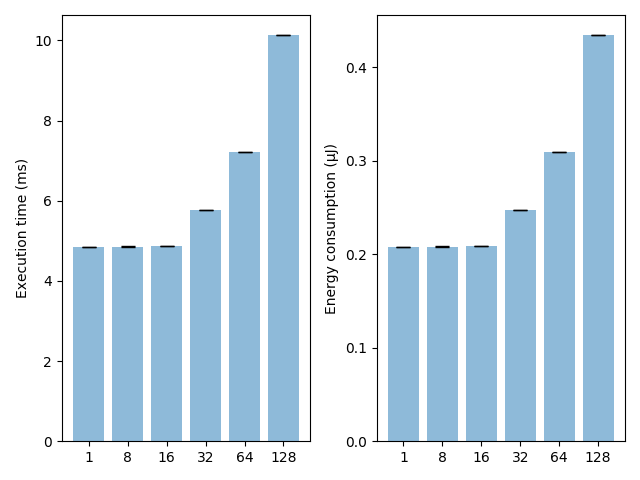
\includegraphics[width=\linewidth]{papers/ppiot/images/iot_bar_plot.png}
    \caption{Execution time and energy consumption for encrypting data. The graphs show the mean of the of the execution times and derived energy consumption with a 95\% confidence interval.}
    \label{fig:iot_performance}
\end{figure}

\subsection{Back End Server Performance}
To evaluate how the throughput of a back-end server would be affected by the privacy protection scheme we have measured the time taken to verify $h_0$, furthermore we have measured the time taken to decrypt the data item $d$ including verifying $h_{in}$. The performance was measured running in a single thread. We have measured the for different encrypted payloads $d$; 1,8,16,32 and 64 bytes. The times for a single payload size $d$ varies considerably, we have made 2000 measurements for each payload size. The times can be seen in Figure \ref{fig:java_performance}. 
%When observing the measurements one can see that the execution times vary, we believe this is because of the non-deterministic performance of the Java Runtime Environment and the underlying operating system.
\begin{figure}[H]
    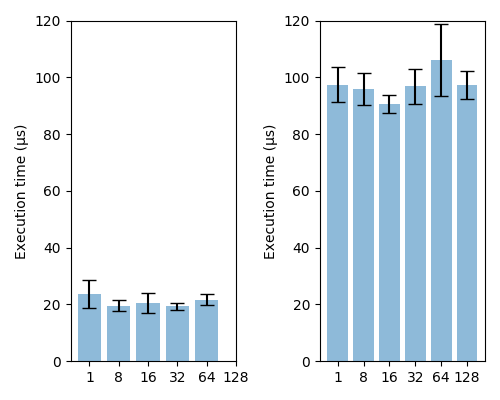
\includegraphics[width=\linewidth]{papers/ppiot/images/java_bar_plot.png}
    \caption{Execution time, left graph shows verifying $h_0$, right graph decryption of encrypted $d$ and verifying $h_{in}$. The graphs show the means of the of the execution times with a 95\% confidence interval.}
    \label{fig:java_performance}
\end{figure}
To give an estimation of the throughput of our solution we use conservative numbers of $50\mu s$ for verifying $h_0$ and $150\mu s$ for decrypting and verifying $d$, this gives us a total time of $200\mu s$ for one data item. The total throughput for one core would then be 5000 data items per second.

\subsection{Memory usage on IoT devices}
IoT devices have limited resources in terms of memory, any scheme developed for such a device must keep this in mind. Here we present numbers for the memory utilization of our implementation. The total utilization of ROM was 2344 Bytes and 426 Bytes of RAM. This was used by SHA256 836 Bytes, HMAC-SHA256 114 Bytes, AES128-CTR 1026 Bytes, Encryption Function 368 Bytes. The RAM was divided between 144 Bytes of keys in RAM and buffers for the encryption process of 282 Bytes. This is manageable amounts of memory needed for such a scheme. If the cipher and hash algorithms would be hardware-accelerated the memory usage would be even lower.


\section{Related work}
\label{relatedwork}
Privacy is a major concern in the IoT paradigm\cite{perera2015big}. People and devices are surrounded by billions of IoT devices gathering zettabytes of data, device manufacturers still do not pay enough attention to privacy while IoT devices are not capable of handling costly solutions to preserve privacy. 

%In  they provide good notions and terminology for iot data privacty, identity data temporal and location etc...

When discussing privacy it is worthwhile to note that there are several types of privacy\cite{porambage2016quest}. Data privacy aims at preserving privacy by not revealing data created or owned by an entity, while identity privacy aims at protecting the identity of a user or entity. There are also the notion of spatial or location privacy, here the goal is to hide or obfuscate the location of the user or entity. This is mostly relevant in the domain of mobile devices\cite{chen2017robustness}  but can also have an impact for V2X networks and IoT networks. Location privacy is not directly related to the work we present in this paper. 

The principle of k-anonymity was first introduced 1998 by  Pierangela and Sweeney and has been extensively use as an annonymization measure in different privacy settings \cite{Sweeney2002}. An overview of different k-anonymity approaches is given in \cite{Ayala2014}. In our paper we adapt the k-anonymity principle in an IoT identity privacy setting.

General privacy-preserving solutions include differential privacy \cite{DworkMNS06}, homomorphic encryption \cite{gentry2009fully}\cite{naehrig2011can}, and secure multi-party computation \cite{bringer2013privacy}. %\cite{lindell2005secure}
Another general line of research which is relevant to IoT is privacy-preserving aggregation of time-series data \cite{JoyeL13}\cite{BenhamoudaJL16}\cite{EmuraKOS18}\cite{ShiCRCS11}.

Many sensors periodically generate data on e.g. temperature and sends it to a server for analysis. A recent summary of these more general problems can be found in \cite{shan2018practical}. Bista et. al. provides a survey of privacy-preserving data aggregation protocols for wireless sensor networks (WSN). In \cite{conti2009privacy}, a scheme for anonymous data transfer using only symmetric key operations is presented. The paper introduces the notion of twin-keys, keys negotiated between two nodes where the nodes does not know the identity of the other node in the pair. This provides anonymity of individual devices when doing data aggregation.

However, all these approaches are so far elusive for the IoT paradigm: they are too computationally costly for resource-constrained IoT devices.  

Going into solutions aimed specifically at IoT it is worth to note that IoT includes a wide spectrum of devices and technology. While different solutions have been proposed for IoT, the work has primarily aimed at data privacy. 
One application of IoT is smart electricity meters (SM), a device measures the electricity consumption at a customer. The measurements needs to be forwarded to the utility-company for billing, but the customers privacy needs to be considered. Learning when the customer utilizes electricity can reveal the users habits. In \cite{Silva:2017:SPP:3019612.3019795} Silva et. al. presents a scheme for data aggregation in smart electricity meters using an Intel SGX enclave to perform the data aggregation while providing end user privacy. 

In \cite{zhang2018data} Zhang et. al. survey the entire fields of security and privacy in edge computing. They give an overview of edge computing, list issues regarding security and privacy, list requirements. They also provide descriptions of key technologies: Identity-based encryption, Attribute-based encryption, proxy re-encryption, homomorphic encryption and searchable encryption. They give an overview of state-of-the-art solutions for data confidentiality, data integrity, privacy preserving and more. They have a section on both data-privacy and identity-privacy, they list some proposed schemes for identity privacy.

Identity privacy has been researched primarily in the fields of Mobile Communications and Vehicular Networks. in the field of Mobile Communications Khan et. al. presents their scheme for dynamic credential generation in \cite{khan2013enhanced}, they also provide an extensive overview of work in the field. Their proposed scheme uses public-key encryption, which makes their proposed solution too computationally intensive for our use-case.

In the field of Vehicular Networks Identity privacy is important\cite{whyte2013security} since a vehicle broadcasting the the identity of the vehicle or driver would enable location tracking of the vehicle or driver. Most of the identity privacy issues of Vehicular networks are solved by pseudonyms, the vehicle is issued with a public-key pair that is periodically changed. Much research has been done on how to improve these schemes \cite{lin2013}, \cite{lin2008tsvc}. However, since the basis of these systems are based on public-key cryptography they are to computationally complex for constrained IoT devices. 

\section{Conclusion and future work}
\label{conclusion}
In this paper, we presented a novel principle for IoT identity protection when using pure symmetric key based data confidentiality and integrity protection. The symmetric key approach has big advantages compare to a public key-based approach as it allows fast analytic processing directly on the protected data items on cloud resources. Identity privacy in this context has not been treated in the literature before and we provided basic security definitions. Using these definition, we presented a novel \textit{combined} identity protection, encryption and integrity protection scheme for IoT data objects. The suggested protection scheme gives not full privacy in all adversary scenarios but, as we view it, gives a fair trade-off between identity protection and complexity. In particular, the proposed schemes uses a two layered protection approach where an ''outer'' protection schemes gives k-anonymity based on symmetric keys shared by several IoT units. If such key would be compromised, an ''inner'' identity protection schemes based on random encryption gives a second level of privacy defense. The security analysis we presented, shows that a reasonable level of identity privacy is achieved with this approach, as long as the adversary not has access to a large number of compromised IoT units or a large number of mappings between specific protected data items and the IoT identity behind the data items. Furthermore, by tuning the protection parameters, increased privacy can be achieved thought the price of more memory usage at the IoT device side. Our proof of concept implementation verifies that the proposed principle indeed offers both low energy consumption encryption at the IoT side as well as fast decryption at the analytic engine side. In future work, we intend to make a full-scale implementation of the approach on IoT data from an industrial control system. In this extended system trial, we will also integrate the solution with a selected set of state-of-the art analytic engines. It is also left for future work to investigate if even more efficient identity privacy preserving schemes for symmetric encryption can be constructed.

{\raggedright
        \printbibliography[segment=\therefsegment,heading=subbibliography]
}

